\documentclass{article}

\usepackage{graphicx}

\addtolength{\oddsidemargin}{-.875in}
\addtolength{\evensidemargin}{-.875in}
\addtolength{\textwidth}{1.75in}
\addtolength{\topmargin}{-.875in}
\addtolength{\textheight}{1.75in}

\begin{document}
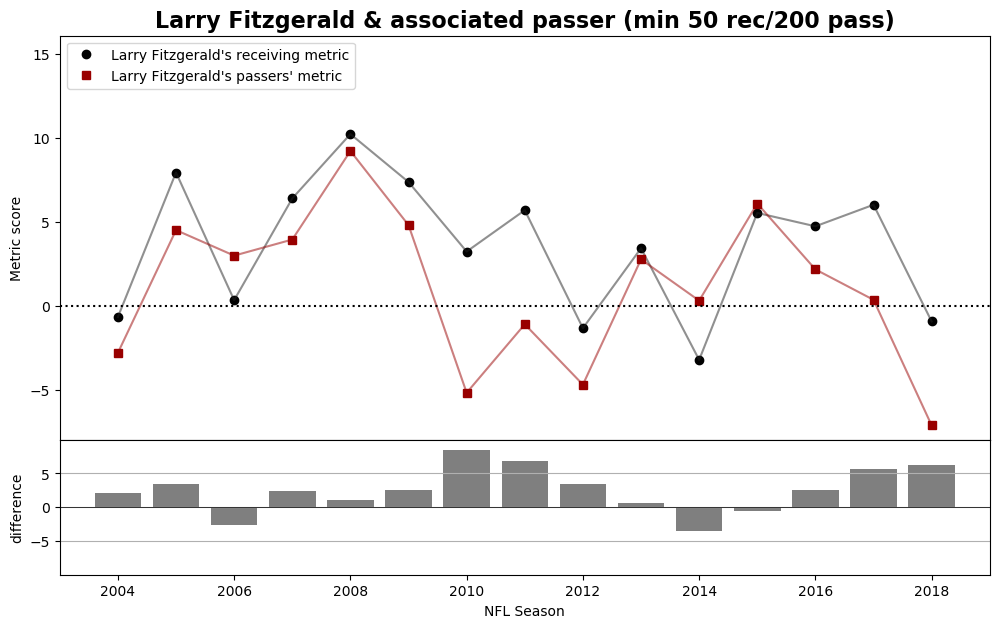
\includegraphics[width=\textwidth]{2506106_metric.pdf}
The following three plots compare the metric scores for receivers (black points) compared to their quarterbacks (red squares).  
The metric is constructed such that the league average among qualifying players (50 receptions or 200 pass attempts) is 0.
The intent of the metric is to see if a receiver ``outperforms'' the play of his quarterback.
The lower bar plot shows the difference between the receiver and the quarterback metric.

In this example, Larry Fitzgerald of the Arizona Cardinals is a model of consistency through many quarterback changes, from Kurt Warner's excellent 2007-2009 seasons, to six different quarterbacks from 2010-2012, and Carson Palmer's arrival in 2013.
While Fitzgerald's production did dip at times (particularly in 2014), he typically performed above the level of his quarterback by this metric.
A player with this type of plot would be a safe bet to be consistently productive despite changes the level of his quarterback's play.

\newpage
\includegraphics[width=\textwidth]{2495821_metric.pdf}
Here we have the opposite case in Marques Colston, the former Saints receiver.
While certainly a very good receiver, he had the luxury of playing alongside Drew Brees---one of the most prolific passers ever from a statistics standpoint---for his entire career.
Colston's metric score is consistently lower than his quarterback's, while there are examples of receivers matching or even surpassing exceptional quarterbacks' annual metric scores (such as Fitzgerald's 2008 season in the previous example).
As such, Colston is an example of a player where it would be wise to question his production on another team or with a different quarterback.

\newpage
\includegraphics[width=\textwidth]{2508061_metric.pdf}
Despite playing with a solidly above average quarterback in Ben Roethlisberger, Antonio Brown's receiving metric scores after 2013 are exceptional, often twice as high as his quarterback's.
Given that he will be playing for a new team and new quarterback in this upcoming season, it is save to expect he will continue to produce at a very high level.

\end{document}
